\subsubsection{ Warping }

We now explain the {\warpunit}. A warp unit generally consists of the following 5 gadgets: \prewarp,
\firstwarp, \warpbridge, \secondwarp, \postwarp. The job of these 5 gadgets is to transport the value
read by the {\tt Counter\_Read} all the way to the digit region in the next row, so that the {\cwrite} gadgets
can write the next value in the correct locations. The {\firstwarp} and {\secondwarp} gadgets are single
tile gadgets that have north and south glues with identical labels. This allows the gadgets to continuously
assemble until stopped by earlier parts of the assembly. These single tile gadgets also have one additional glue
that will allow the next piece in the warp unit to assemble, however the assembly will also block this side of the tile
all the way until the gadget can no longer continue assembling in the north direction.

    \begin{itemize}

        \item {\prewarp}: These gadgets use the bits read from the {\cread} gadgets to translate them into
                          a signal used to tell the counter whether to begin reading
                          another digit in the current row, or cut across the rectangle and begin reading the
                          first digit in the next row. This signal is used from the {\prewarp} gadgets through
                          the {\dtop} gadgets are attached after writing the current digit.

            For each $i = 1,2,3, u \in \{0, 1\}^l$, and each $\inc \in \{ {\tt increment, copy } \}$:
            \begin{itemize}


            \item if $u$ ends with 00:
            create
            $\begin{aligned}[t]
                \prewarp(& \left\langle {\tt PreWarp},   i, u, \inc \right\rangle,
                           \left\langle {\tt FirstWarp}, i, u, \inc \right\rangle \;)
            \end{aligned}$ \\ from the general gadget in Figure~\ref{fig:pre_warp_general}.

            \item if $u$ ends with 01:
            create
            $\begin{aligned}[t]
                \prewarp(& \left\langle {\tt PreWarp},   i, u, \inc \right\rangle,
                           \left\langle {\tt FirstWarp}, i, u, \inc, {\tt msr} \right\rangle \;)
            \end{aligned}$ \\ from the general gadget in Figure~\ref{fig:pre_warp_1_op_msr_msd}.


            \item if $u$ ends with 11 and $dec(u >> 2) >= m$:\\
            create
            $\begin{aligned}[t]
                \prewarp(& \left\langle {\tt PreWarp},   i, u, \inc \right\rangle,
                \left\langle {\tt FirstWarp}, i, u, \inc, {\tt halt},  \right\rangle \;)
            \end{aligned}$ from the general gadget in Figure~\ref{fig:pre_warp_1_op_msr} if $i = 1$ (case 1),
            or Figure~\ref{fig:pre_warp_2_op_msr_msd} if $i = 2$ (case 2), or Figure~\ref{fig:pre_warp_general} if $i = 3$ (case 3).


            \item if $u$ ends with 11:
            create
            $\begin{aligned}[t]
                \prewarp(& \left\langle {\tt PreWarp},   i, u, \inc \right\rangle,
                           \left\langle {\tt FirstWarp}, i, u, \inc, {\tt msr}, {\tt msd} \right\rangle \;)
            \end{aligned}$ from the general gadget in Figure~\ref{fig:pre_warp_1_op_msr} if $i = 1$ (case 1),
            or Figure~\ref{fig:pre_warp_2_op_msr_msd} if $i = 2$ (case 2), or Figure~\ref{fig:pre_warp_general} if $i = 3$ (case 3).
        \end{itemize}
        \vspace{.5cm}

        \begin{figure}[H]
            \centering
            \subcaptionbox{General \label{fig:pre_warp_general}}
            {\makebox[0.24\textwidth][c]{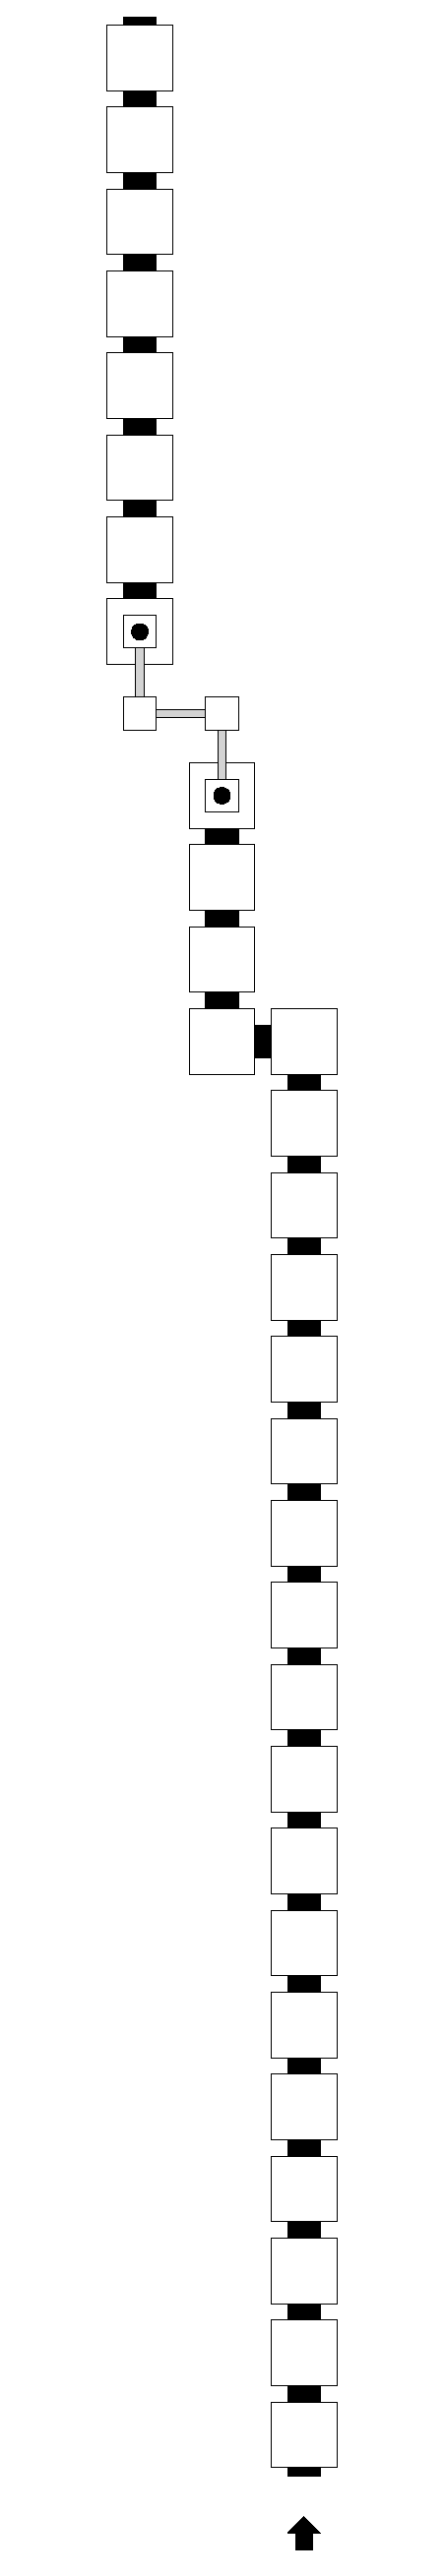
\includegraphics[width=0.11\textwidth]{warping_pre_warp_general}}}%
            ~
            \subcaptionbox{Digit 1 \label{fig:pre_warp_1_op_overview}}
            {\makebox[0.24\textwidth][c]{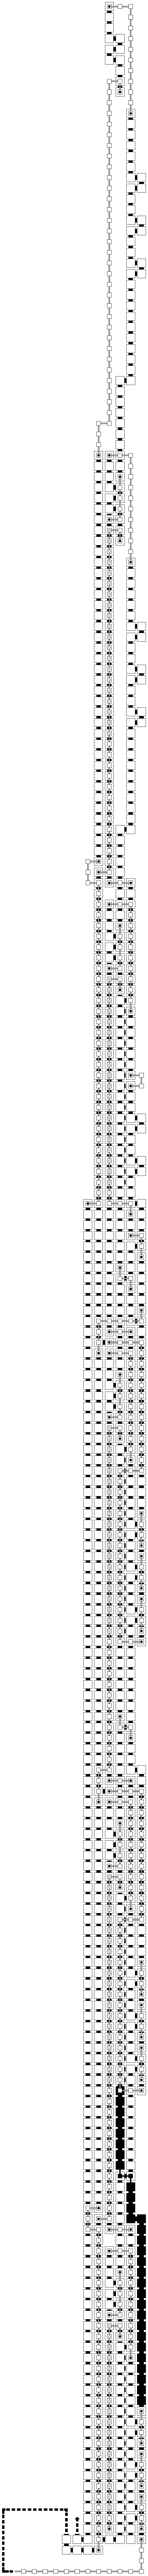
\includegraphics[width=0.45in]{overviews/general/pre_warp_1_op}}}%
            ~
            \subcaptionbox{Digit 2 \label{fig:pre_warp_2_op_overview}}
            {\makebox[0.24\textwidth][c]{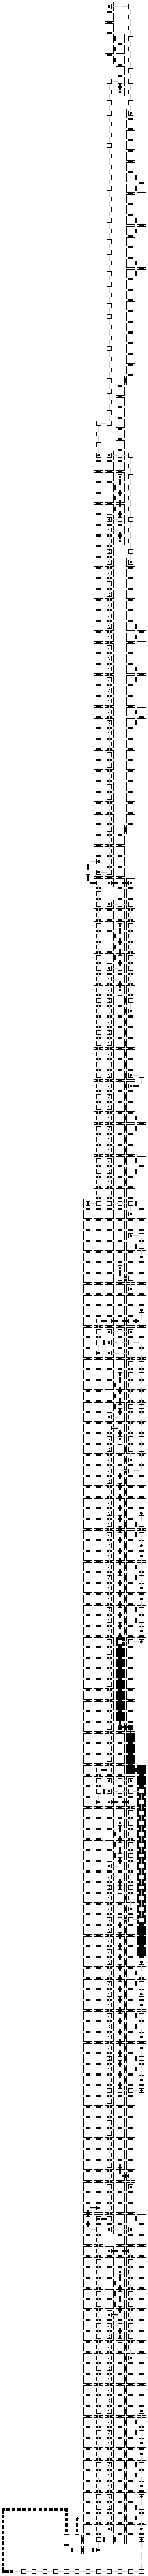
\includegraphics[width=0.45in]{overviews/general/pre_warp_2_op}}}%
            ~
            \subcaptionbox{Digit 3 \label{fig:pre_warp_3_op_overview}}
            {\makebox[0.24\textwidth][c]{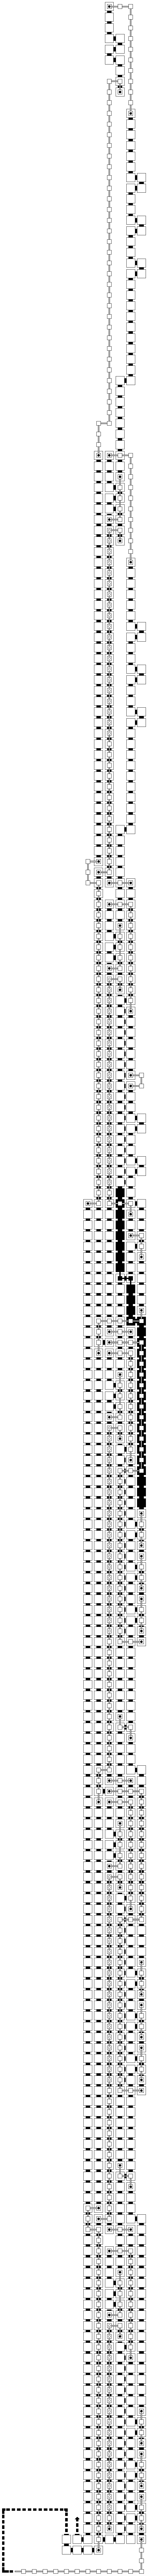
\includegraphics[width=0.45in]{overviews/general/pre_warp_3_op}}}%
            ~
        \end{figure}


        \begin{figure}[H]\ContinuedFloat
            \centering
            \subcaptionbox{Digit 1 -- Case 1 \label{fig:pre_warp_1_op_msr_msd}}
            {\makebox[0.24\textwidth][c]{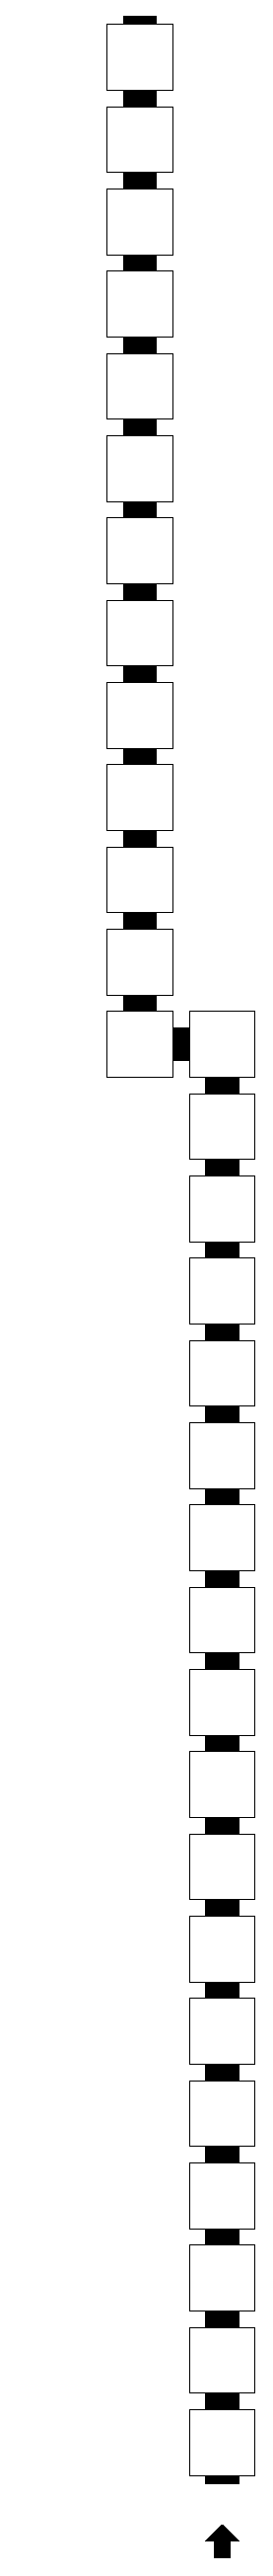
\includegraphics[width=0.33in]{warping_pre_warp_case1_digit1_msr}}}%
            ~
            \subcaptionbox{Digit 1 - Case 1 overview \label{fig:pre_warp_1_op_msr_msd_overview}}
            {\makebox[0.24\textwidth][c]{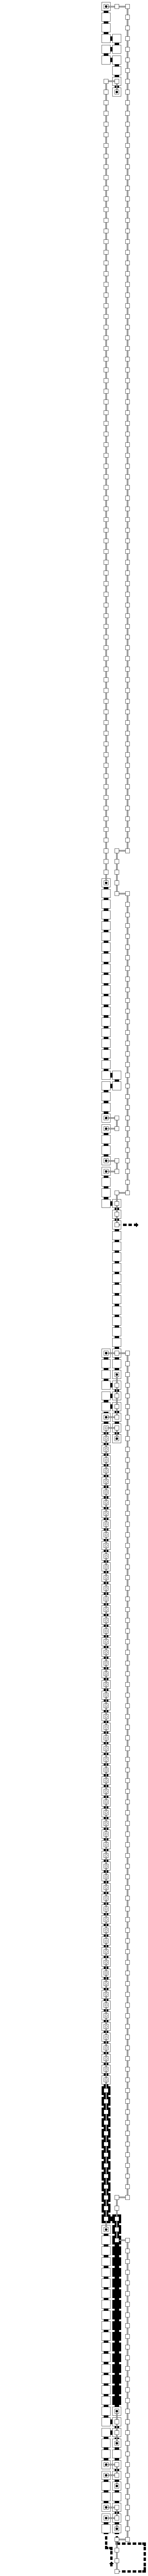
\includegraphics[width=0.45in]{overviews/case1/pre_warp_1_op_msr_msd}}}%
            ~
        \end{figure}

        \begin{figure}[H]\ContinuedFloat
            \centering
            \subcaptionbox{Digit 1 -- Case 2 \label{fig:pre_warp_1_op_msr}}
            {\makebox[0.24\textwidth][c]{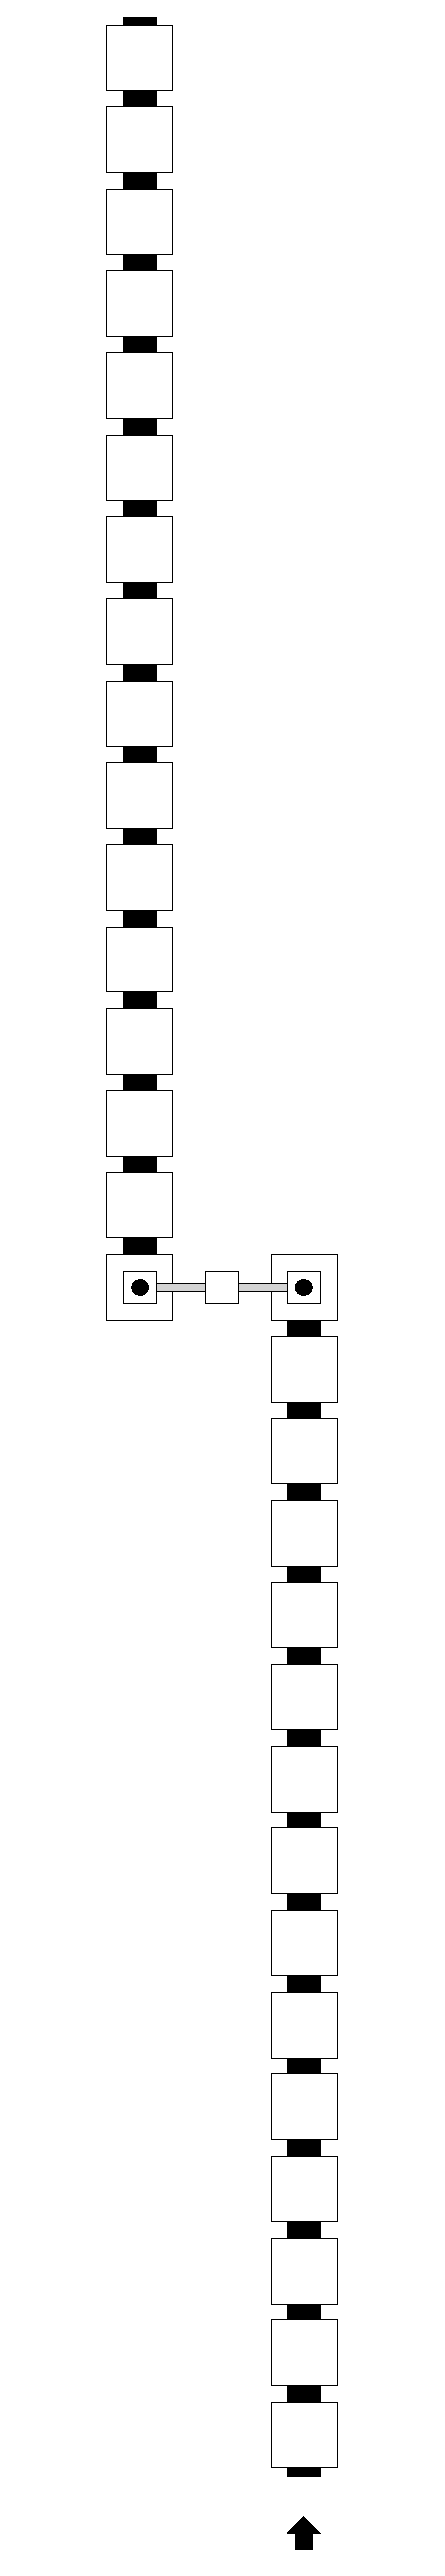
\includegraphics[width=0.33in]{warping_pre_warp_case2_digit1_msr}}}%
            ~
            \subcaptionbox{Digit 1 - Case 2 overview \label{fig:pre_warp_1_op_msr_overview}}
            {\makebox[0.24\textwidth][c]{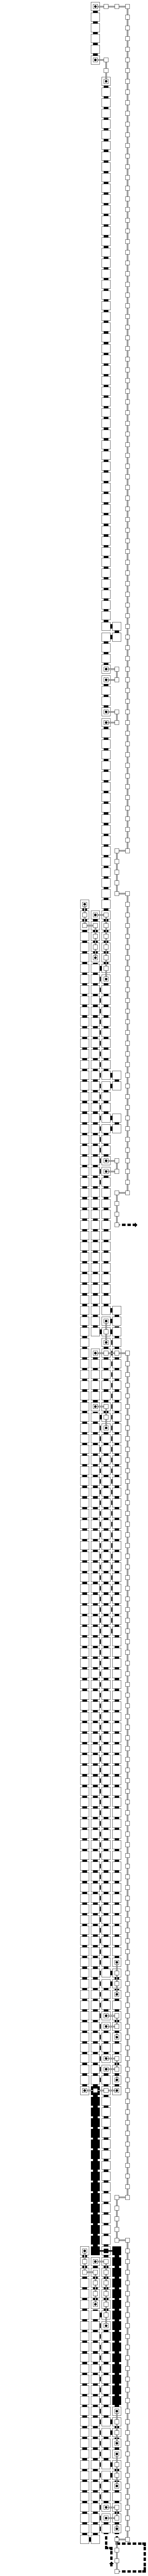
\includegraphics[width=0.45in]{overviews/case2/pre_warp_1_op_msr}}}%
            ~
            \subcaptionbox{Digit 2 -- Case 2\label{fig:pre_warp_2_op_msr_msd}}
            {\makebox[0.24\textwidth][c]{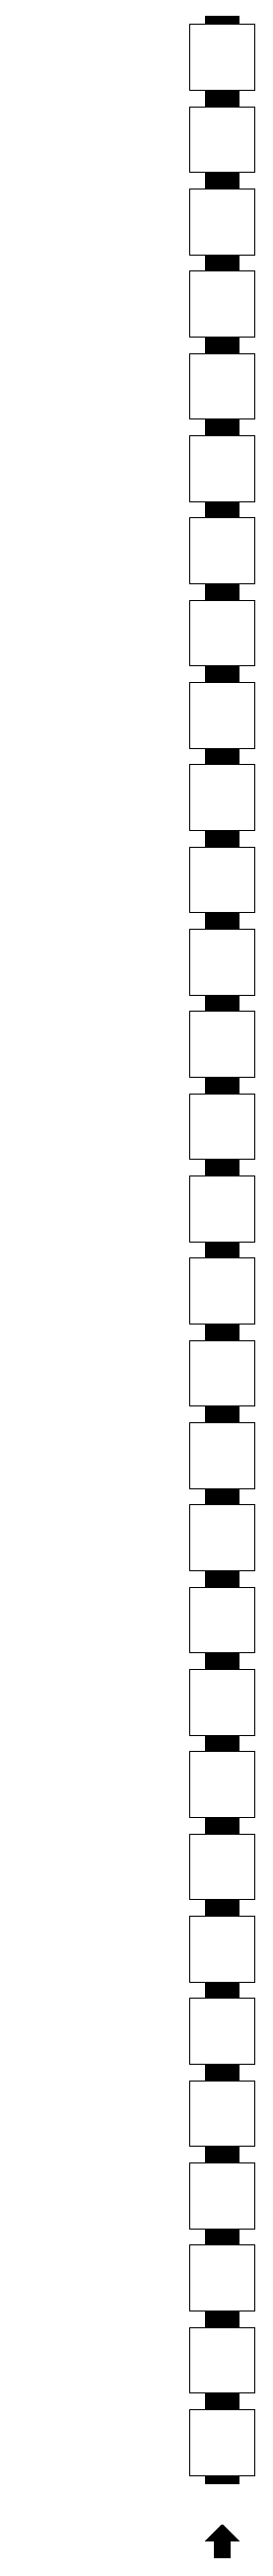
\includegraphics[width=0.33in]{warping_pre_warp_case2_digit2_msr}}}%
            ~
            \subcaptionbox{Digit 2 - Case 2 overview \label{fig:pre_warp_2_op_msr_msd_overview}}
            {\makebox[0.24\textwidth][c]{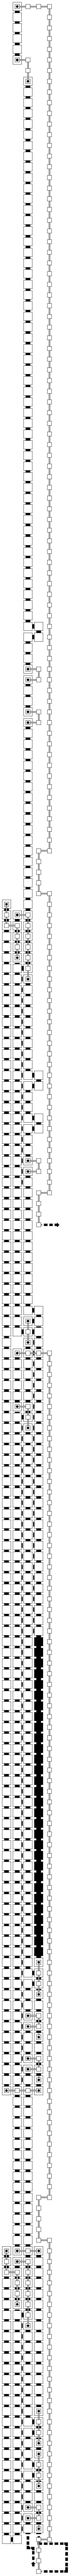
\includegraphics[width=0.45in]{overviews/case2/pre_warp_2_op_msr_msd}}}%
            \caption{\label{fig:pre_warp_gadgets} The {\prewarp} gadgets. }
        \end{figure}


        \item {\firstwarp}: A {\firstwarp} connects to a {\warpbridge} gadget in all cases except when it's assembling
              in the MSR and it is digit 1 in case 1 or 2, in which the {\firstwarp} gadget attaches directly
              to a {\postwarp} gadget.

              For each $u \in \{0, 1\}^l$, and each $\inc \in \{ {\tt increment, copy } \}$:
              \begin{itemize}

                \item For each $i = 1,2,3$: create \\
                $\begin{aligned}[t]
                    \firstwarp(& \left\langle {\tt FirstWarp},  i, u, \inc \right\rangle,    % South
                                 \left\langle {\tt FirstWarp},  i, u, \inc \right\rangle,    % North
                                 \left\langle {\tt WarpBridge}, i, u, \inc \right\rangle \;) % East
                \end{aligned}$
                \vspace{.5cm}

                \item Create
                $\begin{aligned}[t]
                    \firstwarp(& \left\langle {\tt FirstWarp}, 1, u, \inc, {\tt msr} \right\rangle, \\ % South
                               & \left\langle {\tt FirstWarp}, 1, u, \inc, {\tt msr} \right\rangle, \\ % North
                               & \left\langle {\tt PostWarp},  1, u, \inc, {\tt msr} \right\rangle \;) % East
                \end{aligned}$
                \vspace{.5cm}

                \item Create
                $\begin{aligned}[t]
                    \firstwarp(& \left\langle {\tt FirstWarp}, 1, u, \inc, {\tt msr}, {\tt msd} \right\rangle, \\ % South
                               & \left\langle {\tt FirstWarp}, 1, u, \inc, {\tt msr}, {\tt msd} \right\rangle, \\ % North
                               & \left\langle {\tt PostWarp},  1, u, \inc, {\tt msr}, {\tt msd} \right\rangle \;) % Up
                \end{aligned}$
                \vspace{.5cm}

                \item Create
                $\begin{aligned}[t]
                    \firstwarp(& \left\langle {\tt FirstWarp},  2, u, \inc, {\tt msr}, {\tt msd} \right\rangle, \\ % South
                               & \left\langle {\tt FirstWarp},  2, u, \inc, {\tt msr}, {\tt msd} \right\rangle, \\ % North
                               & \left\langle {\tt WarpBridge}, 2, u, \inc, {\tt msr}, {\tt msd} \right\rangle \;) % West
                \end{aligned}$
                \vspace{.5cm}

                \item Create
                $\begin{aligned}[t]
                    \firstwarp(& \left\langle {\tt FirstWarp},  3, u, \inc, {\tt msr}, {\tt msd} \right\rangle,\\  % South
                               & \left\langle {\tt FirstWarp},  3, u, \inc, {\tt msr}, {\tt msd} \right\rangle,\\  % North
                               & \left\langle {\tt WarpBridge}, 3, u, \inc, {\tt msr}, {\tt msd} \right\rangle \;) % East
                \end{aligned}$
                \vspace{.5cm}

            \end{itemize}
            \vspace{.5cm}

        \begin{figure}[H]
            \centering
            \subcaptionbox{Digit 1 overview \label{fig:first_warp_1_op_overview}}
            {\makebox[0.24\textwidth][c]{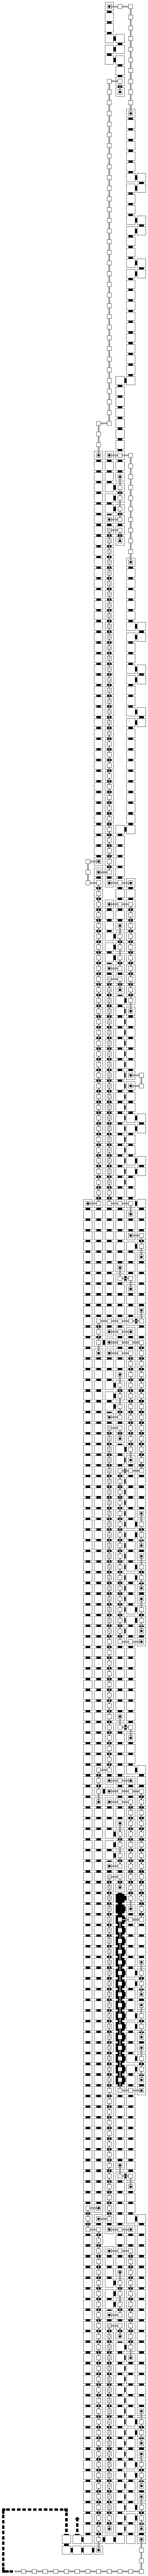
\includegraphics[width=0.45in]{overviews/general/first_warp_1_op}}}%
            ~
            \subcaptionbox{Digit 2 overview \label{fig:first_warp_2_op_overview}}
            {\makebox[0.24\textwidth][c]{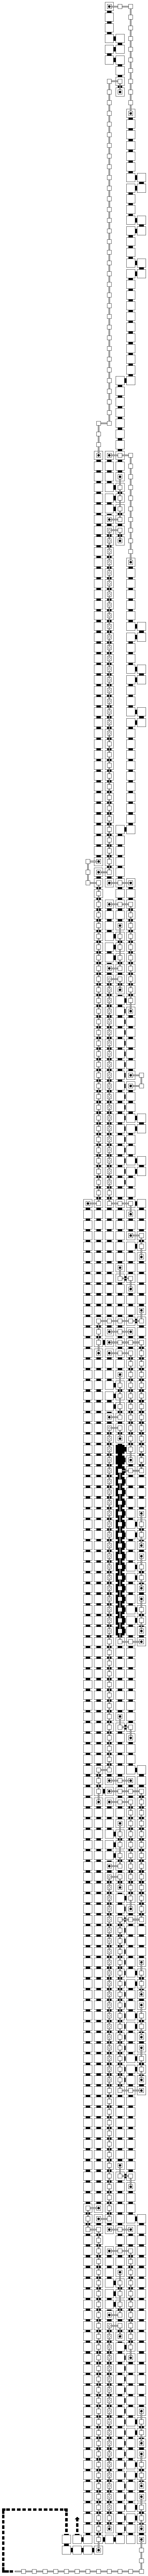
\includegraphics[width=0.45in]{overviews/general/first_warp_2_op}}}%
            ~
            \subcaptionbox{Digit 3 overview \label{fig:first_warp_3_op_overview}}
            {\makebox[0.24\textwidth][c]{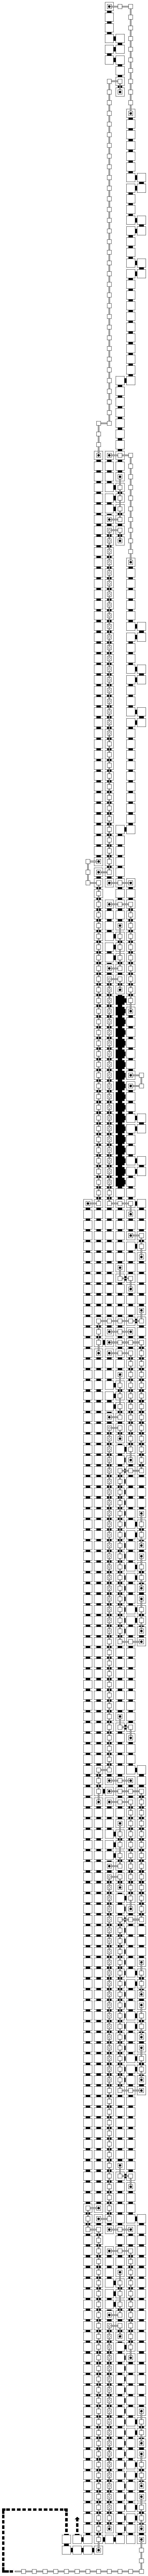
\includegraphics[width=0.45in]{overviews/general/first_warp_3_op}}}%
            ~
            \subcaptionbox{Digit 3 (seed) overview \label{fig:first_warp_3_seed_op_overview}}
            {\makebox[0.24\textwidth][c]{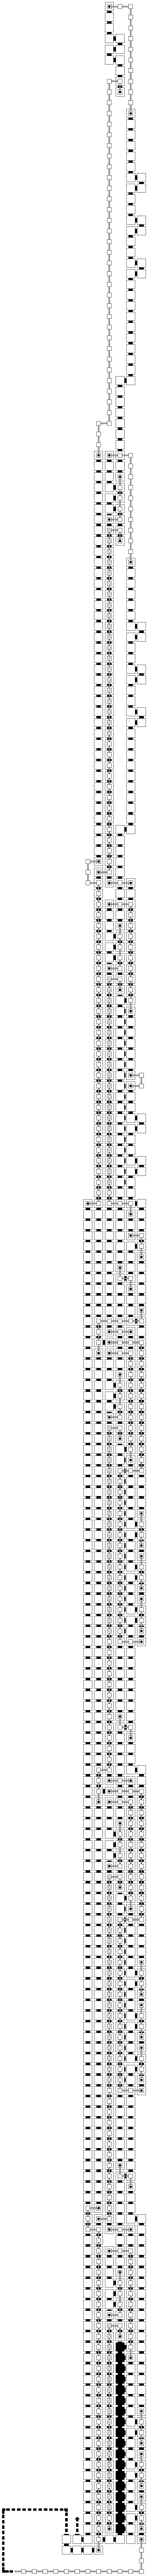
\includegraphics[width=0.45in]{overviews/general/first_warp_3_seed_op}}}%
            ~
        \end{figure}

        \begin{figure}[H]
            \centering
            \subcaptionbox{Digit 1 - case 1 overview \label{fig:first_warp_1_op_msr_msd_overview}}
            {\makebox[0.24\textwidth][c]{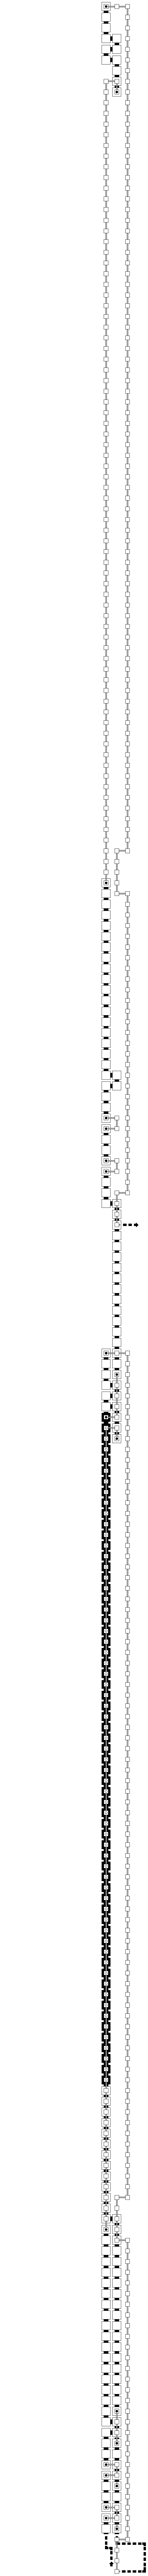
\includegraphics[width=0.45in]{overviews/case1/first_warp_1_op_msr_msd}}}%
            ~
            \subcaptionbox{Digit 1 - case 2 overview \label{fig:first_warp_1_op_msr_overview}}
            {\makebox[0.24\textwidth][c]{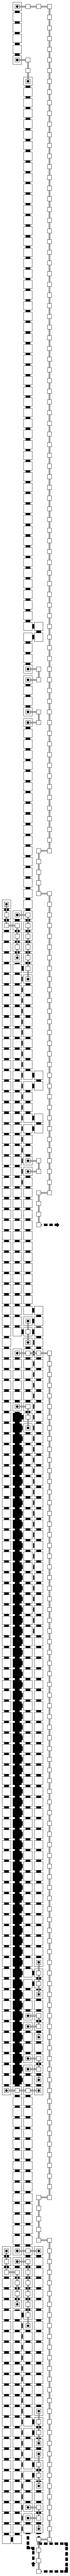
\includegraphics[width=0.45in]{overviews/case2/first_warp_1_op_msr}}}%
            ~
            \subcaptionbox{Digit 2 - case 2 overview \label{fig:first_warp_2_op_msr_msd_overview}}
            {\makebox[0.24\textwidth][c]{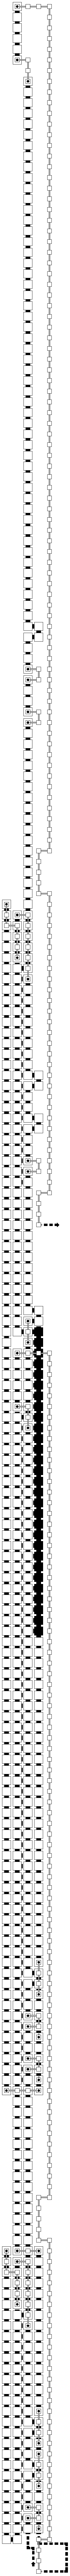
\includegraphics[width=0.45in]{overviews/case2/first_warp_2_op_msr_msd}}}%
            ~
            \caption{\label{fig:first_warp_gadgets_overviews} The {\firstwarp} gadget overviews.}
        \end{figure}


        \item {\warpbridge}: a {\warpbridge} gadget binds the last tile of the {\firstwarp} gadgets to the
             first tile of the {\secondwarp} gadgets. For digit 1 in cases 1 and 2, the
             {\warpbridge} is omitted from the {\warpunit}.

        For each $u \in \{0, 1\}^l$, and each $\inc \in \{ {\tt increment, copy } \}$:
        \begin{itemize}

            \item For each $i = 1,2,3$: create
            $\begin{aligned}[t]
                \warpbridge(& \left\langle {\tt WarpBridge}, i, u, \inc \right\rangle,
                              \left\langle {\tt SecondWarp}, i, u, \inc \right\rangle \;)
            \end{aligned}$ \\ from the general gadget in Figure~\ref{fig:warp_bridge_general}.
            \vspace{.5cm}

            \item Create
            $\begin{aligned}[t]
                \warpbridge(& \left\langle {\tt WarpBridge}, 2, u, \inc, {\tt msr}, {\tt msd} \right\rangle,
                              \left\langle {\tt SecondWarp}, 2, u, \inc, {\tt msr}, {\tt msd} \right\rangle \;)
            \end{aligned}$ \\ from the general gadget in Figure~\ref{fig:warp_bridge_2_op_msr_msd}.
            \vspace{.5cm}

            \item Create
            $\begin{aligned}[t]
                \warpbridge(& \left\langle {\tt WarpBridge}, 3, u, \inc, {\tt msr}, {\tt msd} \right\rangle,
                              \left\langle {\tt SecondWarp}, 3, u, \inc, {\tt msr}, {\tt msd} \right\rangle \;)
            \end{aligned}$ \\ from the general gadget in Figure~\ref{fig:warp_bridge_general}.
            \vspace{.5cm}
        \end{itemize}


        \begin{figure}[H]
            \centering
            \subcaptionbox{General \label{fig:warp_bridge_general}}
            {\makebox[0.11\textwidth][c]{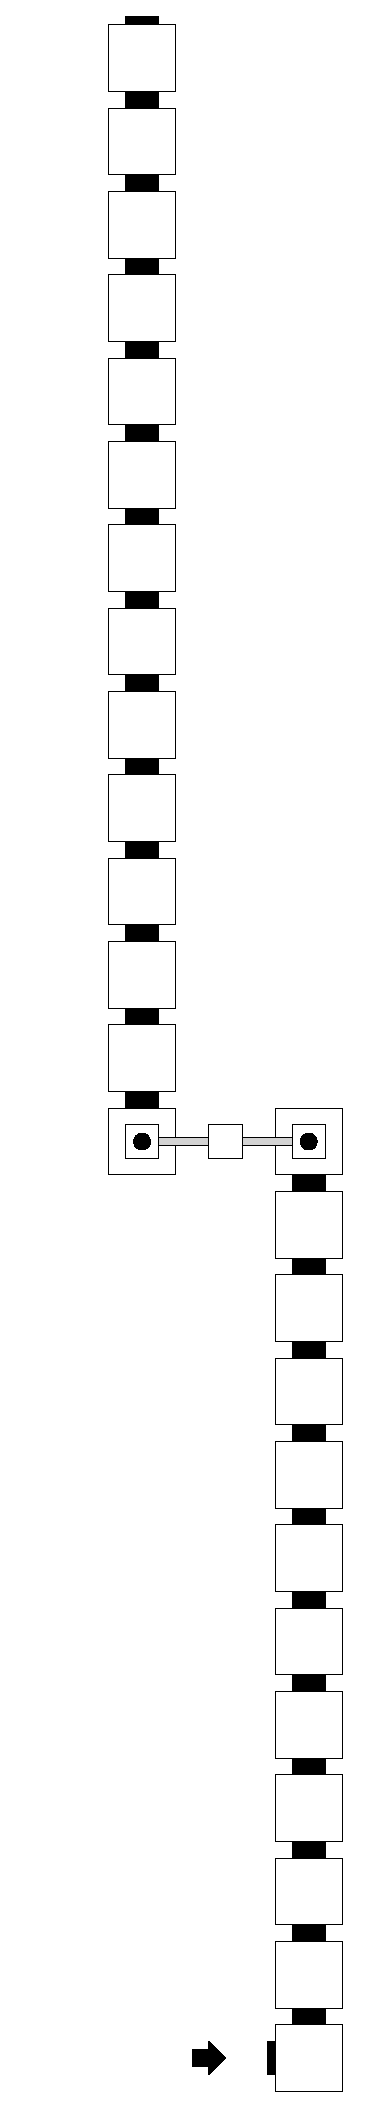
\includegraphics[width=0.33in]{warping_warp_bridge_general}}}%
            ~
            \subcaptionbox{Digit 1 - general overview\label{fig:warp_bridge_1_op_overview}}
            {\makebox[0.19\textwidth][c]{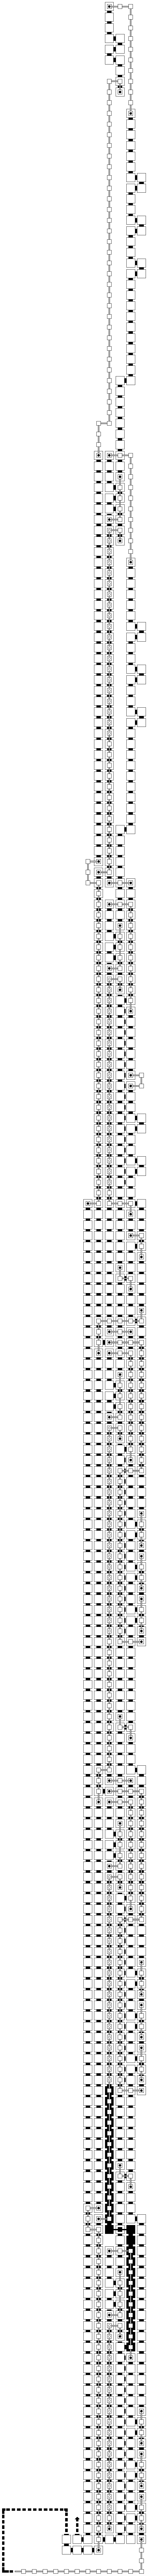
\includegraphics[width=0.45in]{overviews/general/warp_bridge_1_op}}}%
            ~
            \subcaptionbox{Digit 2 - general overview\label{fig:warp_bridge_2_op_overview}}
            {\makebox[0.19\textwidth][c]{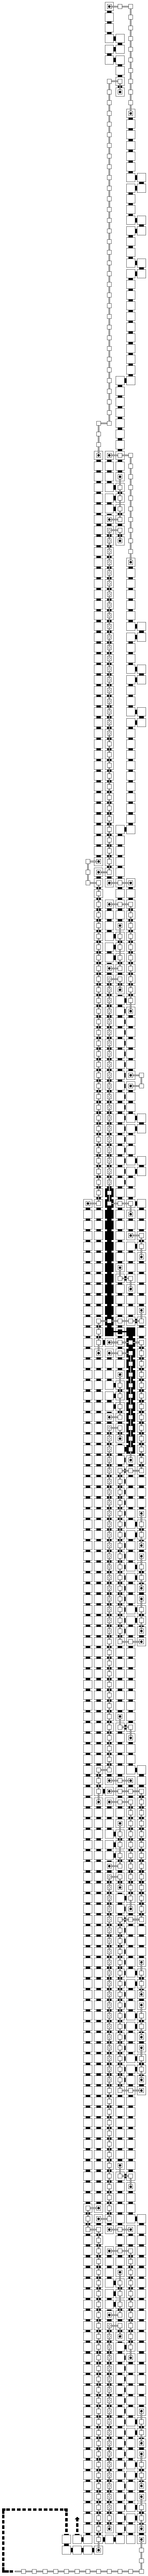
\includegraphics[width=0.45in]{overviews/general/warp_bridge_2_op}}}%
            ~
            \subcaptionbox{Digit 3 - general overview\label{fig:warp_bridge_3_op_overview}}
            {\makebox[0.19\textwidth][c]{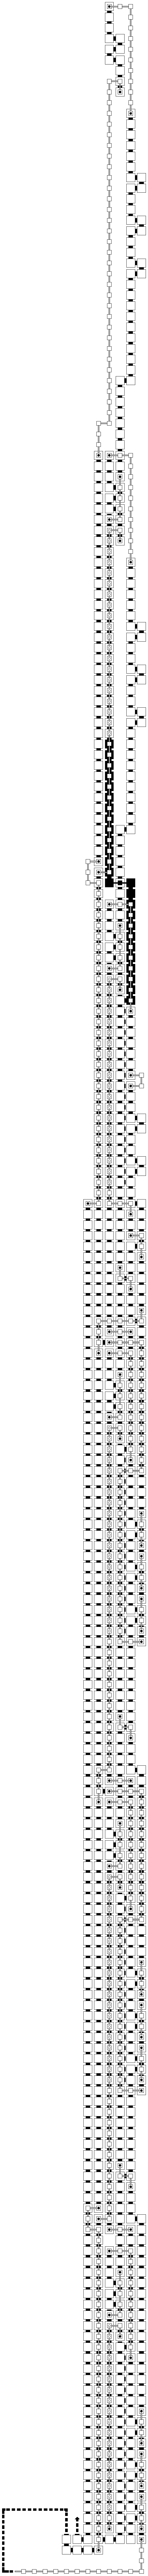
\includegraphics[width=0.45in]{overviews/general/warp_bridge_3_op}}}%
            ~
        \end{figure}

        \begin{figure}[H]\ContinuedFloat
            \centering
            ~
            \subcaptionbox{Digit 2 - general (seed) overview\label{fig:warp_bridge_2_seed_op_overview}}
            {\makebox[0.19\textwidth][c]{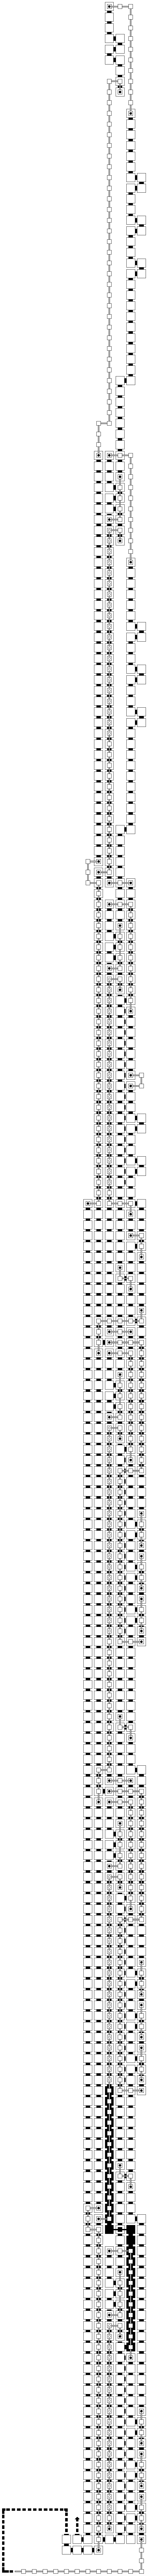
\includegraphics[width=0.45in]{overviews/general/warp_bridge_2_seed_op}}}%
            ~
            \subcaptionbox{Digit 3 - general (seed) overview\label{fig:warp_bridge_3_seed_op_overview}}
            {\makebox[0.19\textwidth][c]{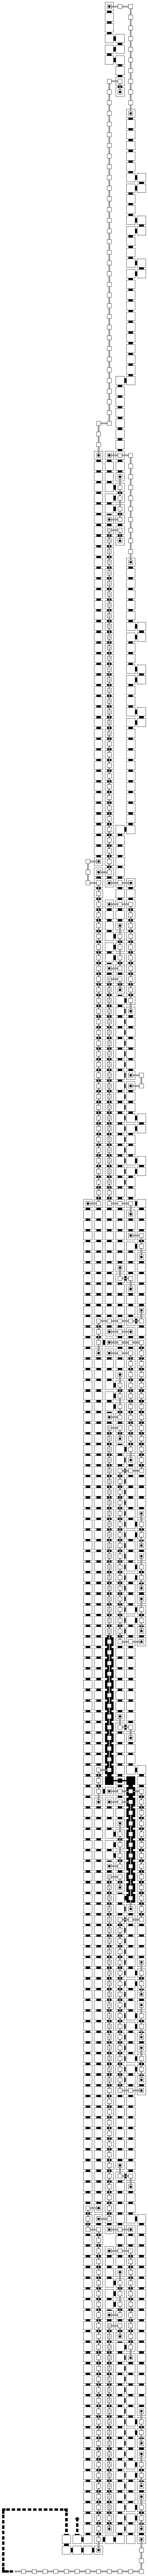
\includegraphics[width=0.45in]{overviews/general/warp_bridge_3_seed_op}}}%
            ~
            \subcaptionbox{Digit 2 \label{fig:warp_bridge_2_op_msr_msd}}
            {\makebox[0.11\textwidth][c]{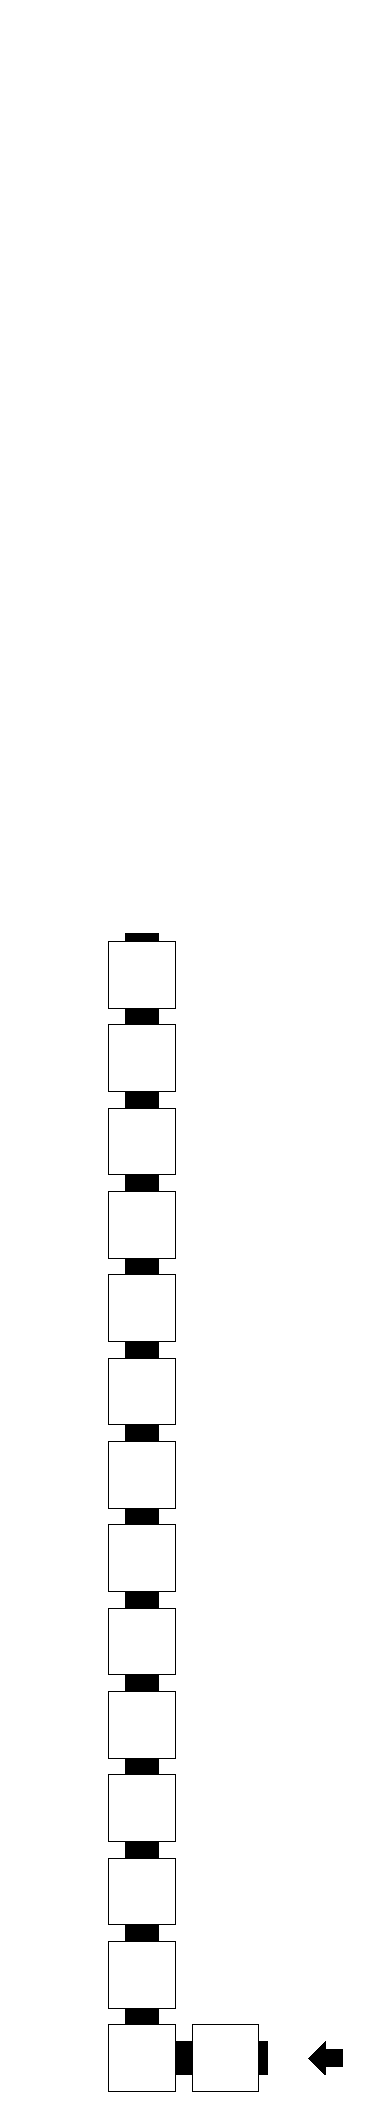
\includegraphics[width=0.33in]{warping_warp_bridge_case2_digit2_msr}}}%
            ~
            \subcaptionbox{Digit 2 - case 2 overview \label{fig:warp_bridge_2_op_msr_msd_overview}}
            {\makebox[0.24\textwidth][c]{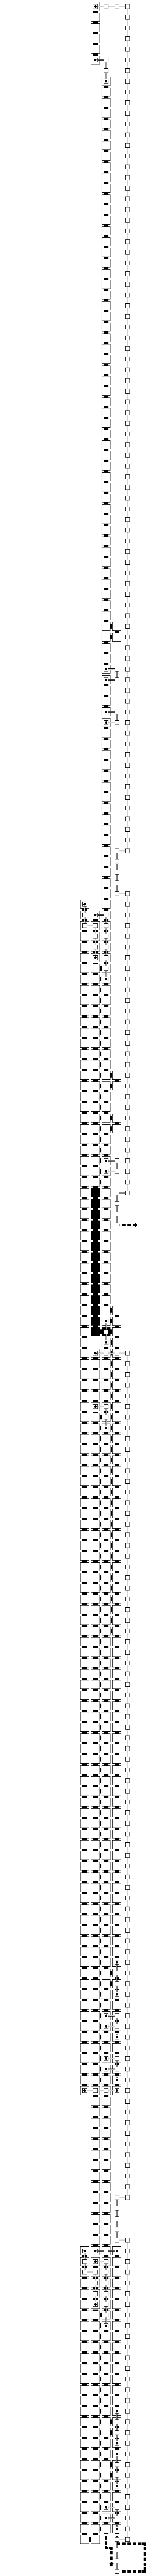
\includegraphics[width=0.45in]{overviews/case2/warp_bridge_2_op_msr_msd}}}%
            ~
            \caption{\label{fig:warp_bridge_gadgets_overviews} The {\warpbridge} gadgets.}
        \end{figure}

        \item {\secondwarp}:
        % The idea of the Second_Warp gadget is to transport the information read by the Counter_Read
        % gadgets, usually across a distance  O(log m). We do this using a single tile that
        % assembles an infinite line in the north direction, and has one unique glue either on the
        % east direction or up direction. This unique glue will at some point, in a unique location that is
        % determined by earlier parts of the assembly, no longer be blocked and so that it can
        % finally attach to the Post_Warp gadget. This process signifies the "waking up" of the
        % Second_Warp gadgets. When this gadget wakes up, it must also be blocked in the north direction, to
        % prevent a truly infinite line from assembling. The geometry required for this process is guarenteed
        % to be in place by earlier-assembled Digit_Top gadgets.


        For each $u \in \{0, 1\}^l$, and each $\inc \in \{ {\tt increment, copy } \}$:
        \begin{itemize}
            \item For each $i = 1, 2, 3$: Create
            $\begin{aligned}[t]
                \secondwarp(& \left\langle {\tt SecondWarp}, i, u, \inc \right\rangle,   \\ % South
                            & \left\langle {\tt SecondWarp}, i, u, \inc \right\rangle,   \\ % North
                            & \left\langle {\tt PostWarp},   i, u, \inc \right\rangle \;)   % Up
            \end{aligned}$

            \vspace{0.5cm}

            \item Create
            $\begin{aligned}[t]
                \secondwarp(& \left\langle {\tt SecondWarp}, 2, u, \inc, {\tt msr}, {\tt msd} \right\rangle, \\ % South
                            & \left\langle {\tt SecondWarp}, 2, u, \inc, {\tt msr}, {\tt msd} \right\rangle, \\ % North
                            & \left\langle {\tt PostWarp},   2, u, \inc, {\tt msr}, {\tt msd} \right\rangle \;) % East
            \end{aligned}$
            \vspace{0.5cm}

            \item Create
            $\begin{aligned}[t]
                \secondwarp(& \left\langle {\tt SecondWarp}, 3, u, \inc, {\tt msr}, {\tt msd} \right\rangle, \\ % South
                            & \left\langle {\tt SecondWarp}, 3, u, \inc, {\tt msr}, {\tt msd} \right\rangle, \\ % North
                            & \left\langle {\tt PostWarp},   3, u, \inc, {\tt msr}, {\tt msd} \right\rangle \;) % Up
            \end{aligned}$
        \end{itemize}

        \begin{figure}[H]
            \centering
            \subcaptionbox{Digit 1 - general\\ overview \label{fig:second_warp_1_op_overview}}
            {\makebox[0.24\textwidth][c]{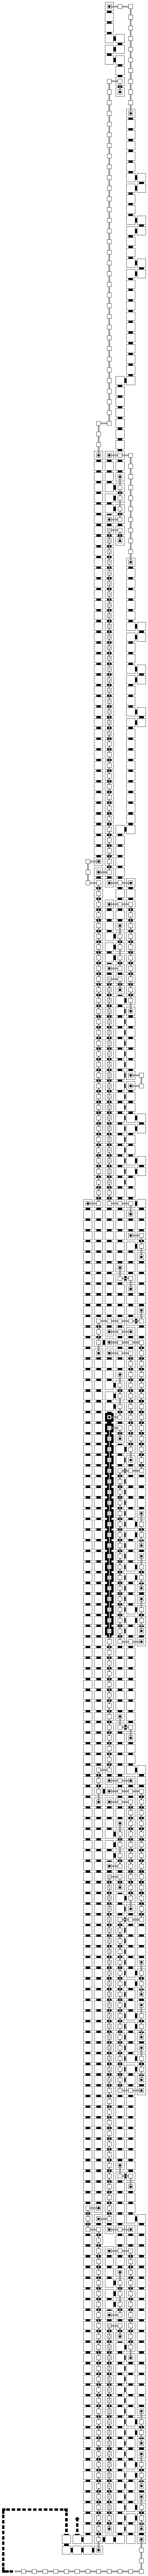
\includegraphics[width=0.45in]{overviews/general/second_warp_1_op}}}%
            ~
            \subcaptionbox{Digit 2 - general\\ overview \label{fig:second_warp_2_op_overview}}
            {\makebox[0.24\textwidth][c]{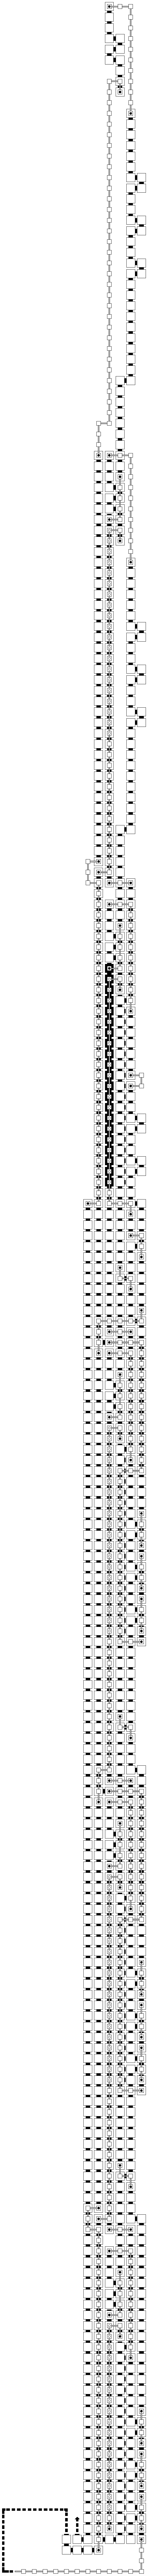
\includegraphics[width=0.45in]{overviews/general/second_warp_2_op}}}%
            ~
            \subcaptionbox{Digit 3 - general\\ overview \label{fig:second_warp_3_op_overview}}
            {\makebox[0.24\textwidth][c]{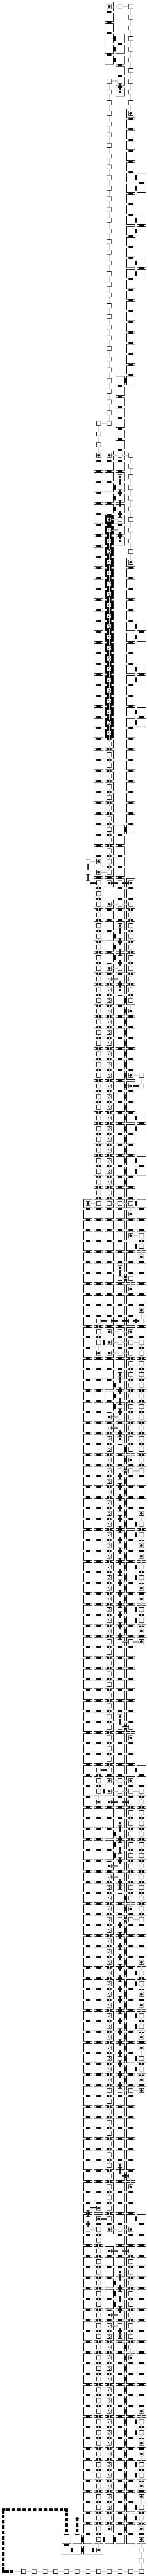
\includegraphics[width=0.45in]{overviews/general/second_warp_3_op}}}%
            ~
            \subcaptionbox{Digit 2 - general (seed) overview \label{fig:second_warp_2_seed_op_overview}}
            {\makebox[0.24\textwidth][c]{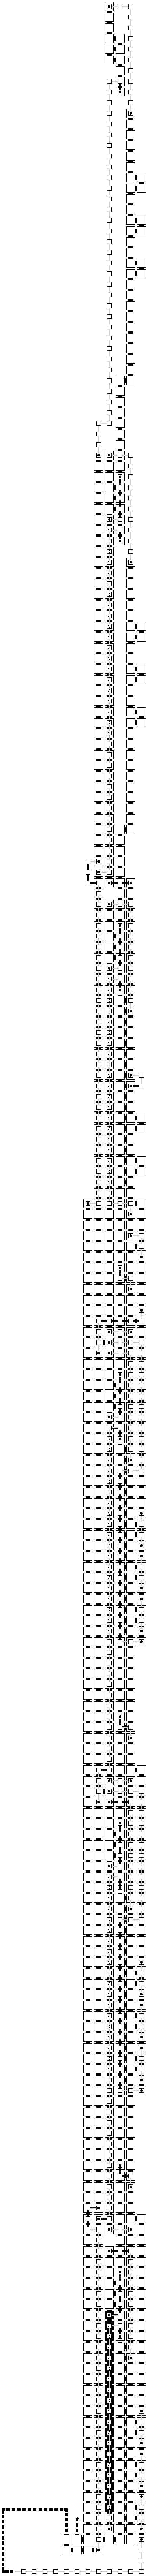
\includegraphics[width=0.45in]{overviews/general/second_warp_2_seed_op}}}%
            ~
        \end{figure}
        \begin{figure}[H]\ContinuedFloat
            \centering
            \subcaptionbox{Digit 3 - general (seed) overview \label{fig:second_warp_3_seed_op_overview}}
            {\makebox[0.24\textwidth][c]{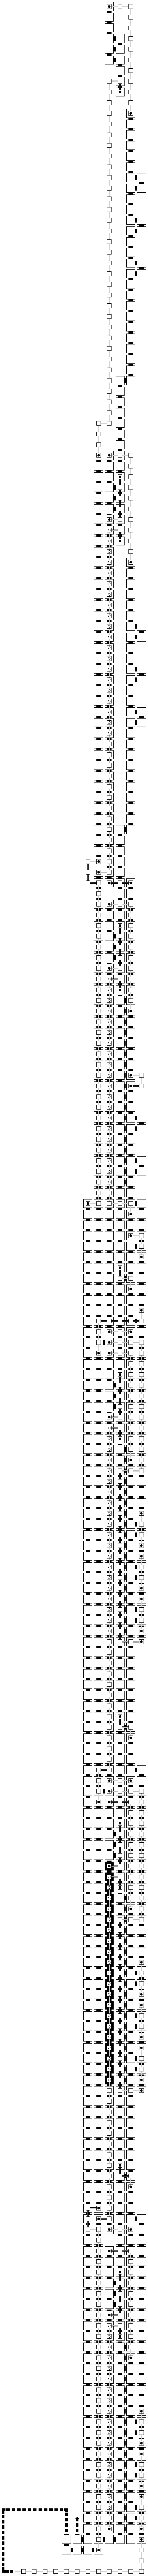
\includegraphics[width=0.45in]{overviews/general/second_warp_3_seed_op}}}%
            ~
            \subcaptionbox{Digit 2 - case 2 overview \label{fig:second_warp_2_op_msr_msd}}
            {\makebox[0.24\textwidth][c]{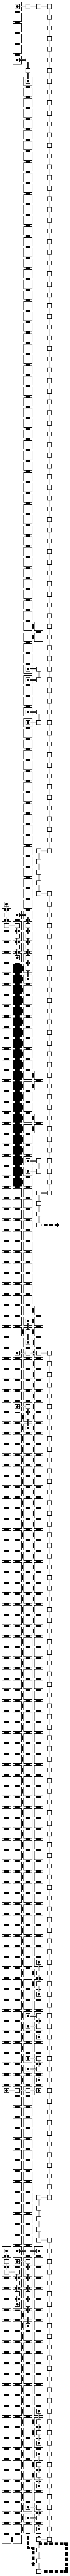
\includegraphics[width=0.45in]{overviews/case2/second_warp_2_op_msr_msd}}}%
            ~
            \subcaptionbox{Digit 2 - case 2 (seed) overview \label{fig:second_warp_2_seed_op_msr_msd_overview}}
            {\makebox[0.24\textwidth][c]{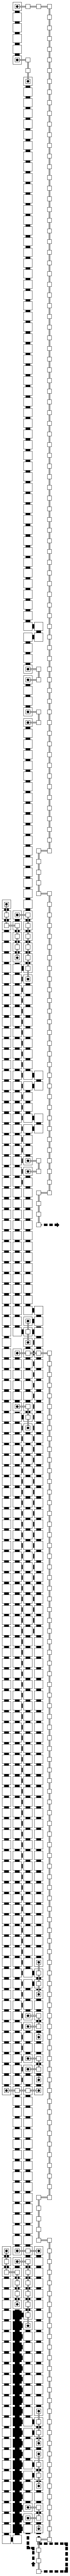
\includegraphics[width=0.45in]{overviews/case2/second_warp_2_seed_op_msr_msd}}}%
            ~
            \caption{\label{fig:second_warp_gadgets_overviews} The {\secondwarp} gadgets overviews.}
        \end{figure}


        \item {\postwarp}:
        \begin{itemize}
           \item For each $i = 1,2,3$: create\\
            $\begin{aligned}[t]
                \postwarp(& \left \langle {\tt PostWarp}, i, u, \inc \right\rangle,    % Down
                            \left \langle {\tt Write},    i, u, \inc \right\rangle \;) % North
            \end{aligned}$ \\
            from the general gadget shown in Figure~\ref{fig:post_warp_1_op} if $i = 1$,
            or Figure~\ref{fig:post_warp_2or3_op} if $ i = 2$ or $i = 3$.
            \vspace{.5cm}


            \item Create
            $\begin{aligned}[t]
                \postwarp(& \left \langle {\tt PostWarp}, 1, u, \inc, {\tt msr} \right\rangle,    % West
                            \left \langle {\tt Write},    1, u, \inc, {\tt msr} \right\rangle \;) % North
            \end{aligned}$ \\
            from the general gadget in Figure~\ref{fig:post_warp_1_op_msr}.
            \vspace{.5cm}

            \item For each $i=1,2,3$: create\\
            $\begin{aligned}[t]
                \postwarp(& \left \langle {\tt PostWarp}, i, u, \inc, {\tt msr}, {\tt msd} \right\rangle,    % Down if i=1 or i=3, West if i=2
                            \left \langle {\tt Write},    i, u, \inc, {\tt msr}, {\tt msd} \right\rangle \;) % North
            \end{aligned}$ \\
            from the general gadget shown in Figure~\ref{fig:post_warp_1_op_msr_msd} if $i = 1$, or
            Figure~\ref{fig:post_warp_2_op_msr_msd} if $i = 2$, or Figure~\ref{fig:post_warp_2or3_op} if $i = 3$.
            \vspace{.5cm}

        \end{itemize}

        \begin{figure}[H]
            \centering
            \subcaptionbox{Digit 1 - general\label{fig:post_warp_1_op}}
            {\makebox[0.19\textwidth][c]{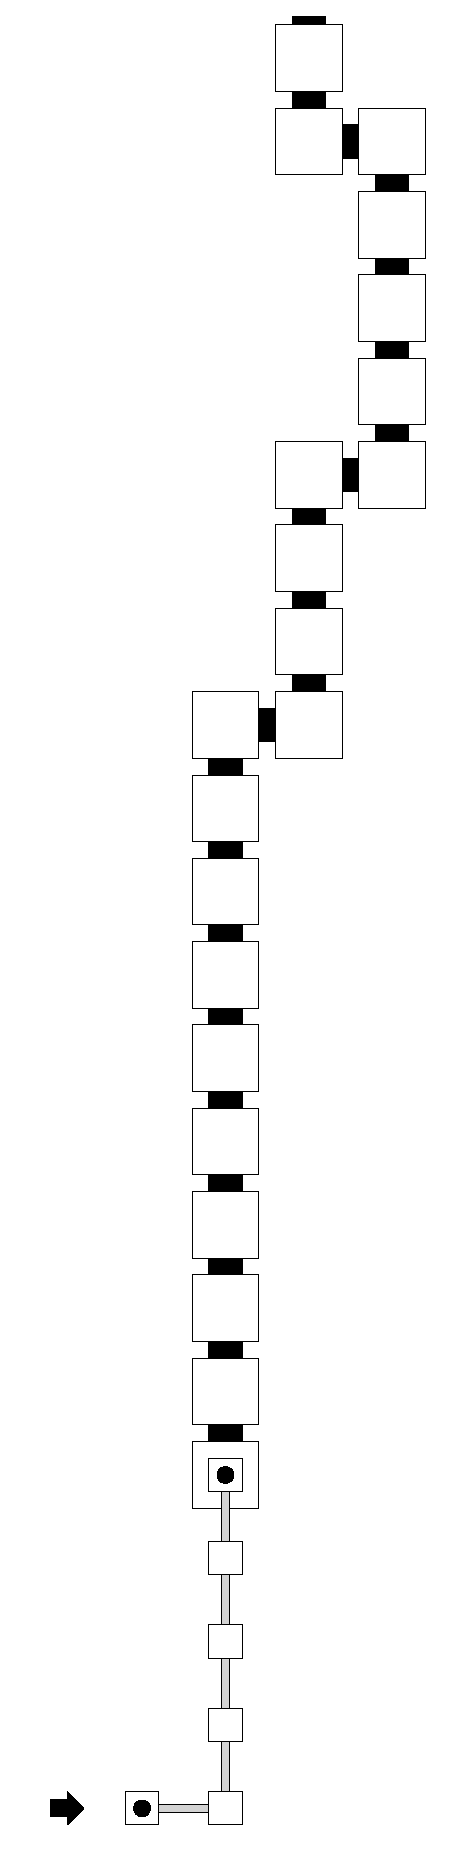
\includegraphics[width=0.45in]{warping_post_warp_general_digit1}}}%
            ~
            \subcaptionbox{Digit 1 - general overview \label{fig:post_warp_1_op_overview}}
            {\makebox[0.19\textwidth][c]{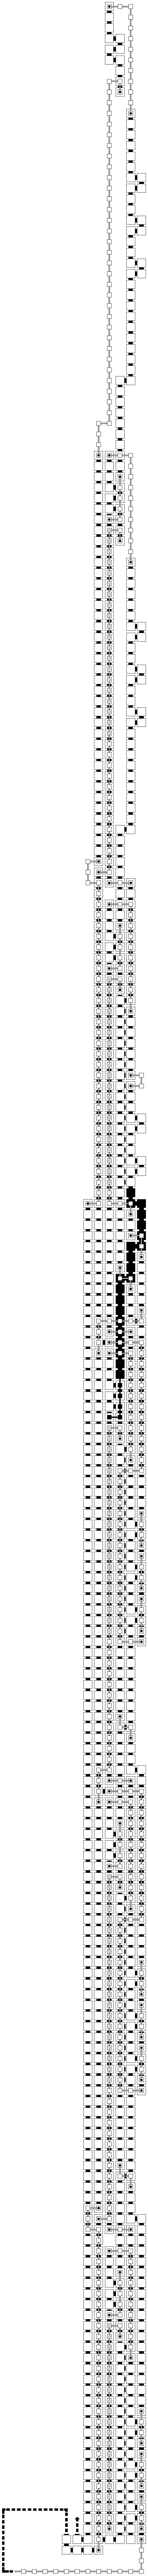
\includegraphics[width=0.45in]{overviews/general/post_warp_1_op}}}%
            ~
            \subcaptionbox{Digit 2 - general \label{fig:post_warp_2or3_op}}
            {\makebox[0.19\textwidth][c]{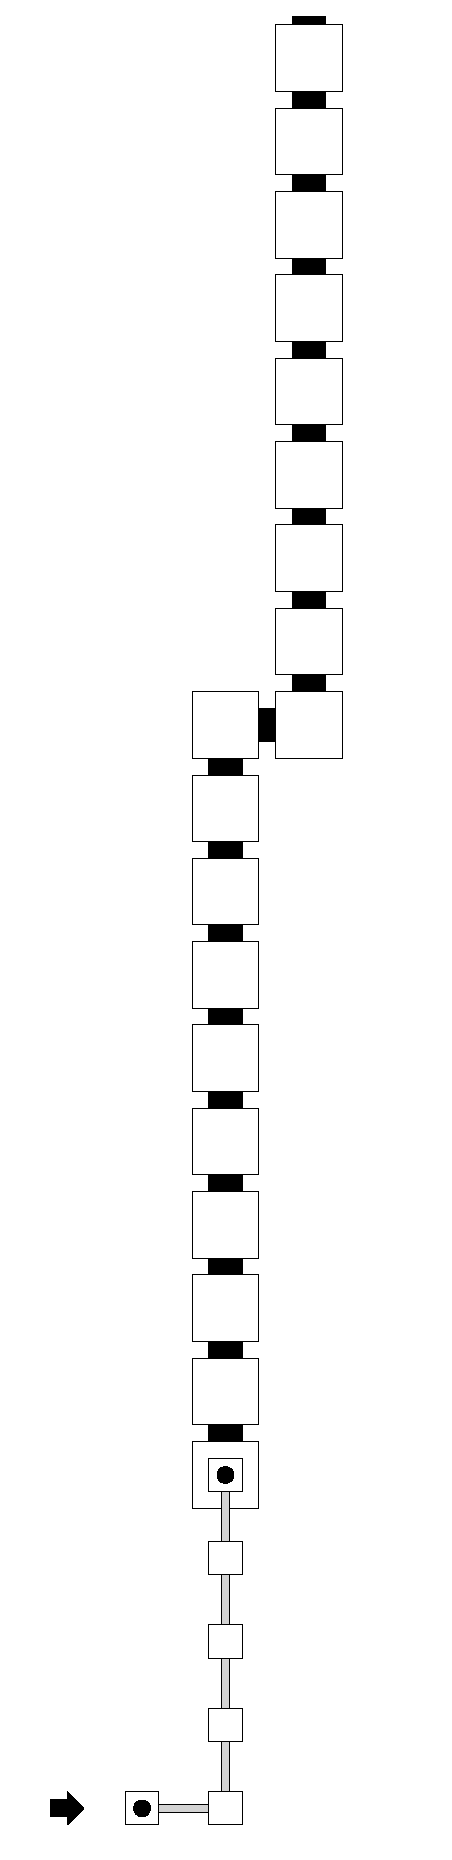
\includegraphics[width=0.45in]{warping_post_warp_general_digit2and3}}}%
            ~
            \subcaptionbox{Digit 2 - general overview \label{fig:post_warp_2_op_overview}}
            {\makebox[0.19\textwidth][c]{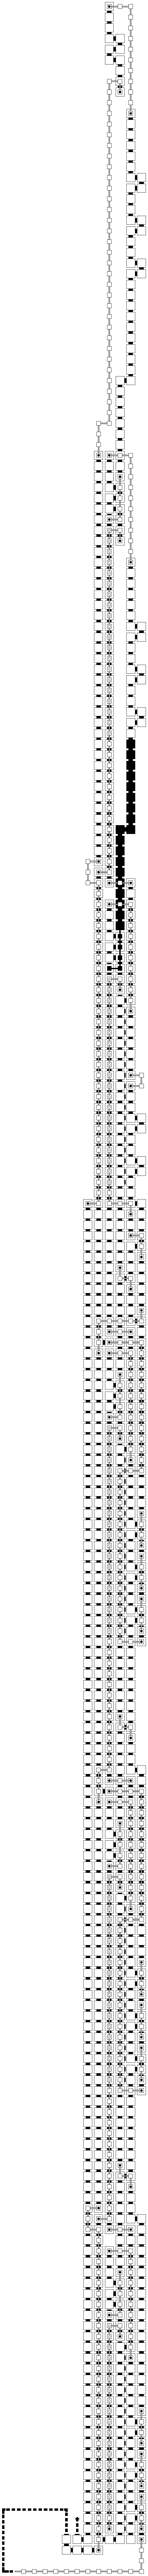
\includegraphics[width=0.45in]{overviews/general/post_warp_2_op}}}%
            ~
            \subcaptionbox{Digit 3 - general overview \label{fig:post_warp_3_op_overview}}
            {\makebox[0.19\textwidth][c]{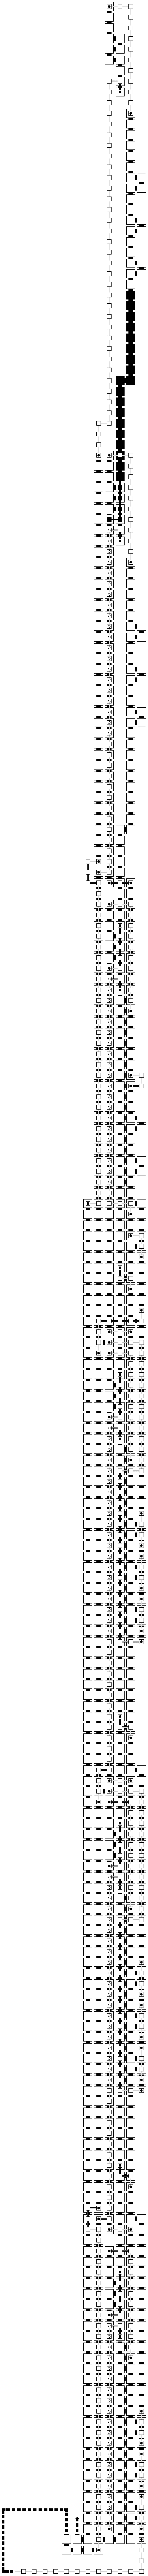
\includegraphics[width=0.45in]{overviews/general/post_warp_3_op}}}%
            ~
        \end{figure}
        \begin{figure}[H]\ContinuedFloat
            \subcaptionbox{Digit 2 - general (seed) overview \label{fig:post_warp_2_seed_op_overview}}
            {\makebox[0.24\textwidth][c]{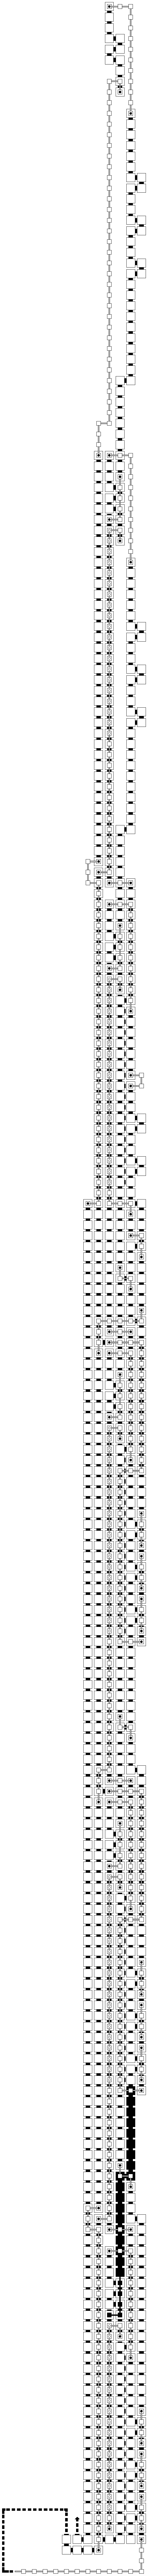
\includegraphics[width=0.45in]{overviews/general/post_warp_2_seed_op}}}%
            ~
            \subcaptionbox{Digit 3 - general (seed) overview \label{fig:post_warp_3_seed_op_overview}}
            {\makebox[0.24\textwidth][c]{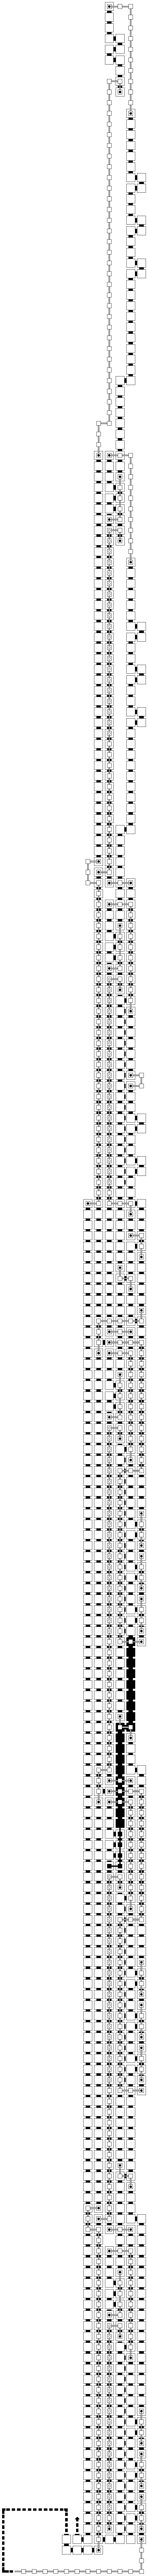
\includegraphics[width=0.45in]{overviews/general/post_warp_3_seed_op}}}%
            ~
            \subcaptionbox{Digit 1 - case 1 \label{fig:post_warp_1_op_msr_msd}}
            {\makebox[0.24\textwidth][c]{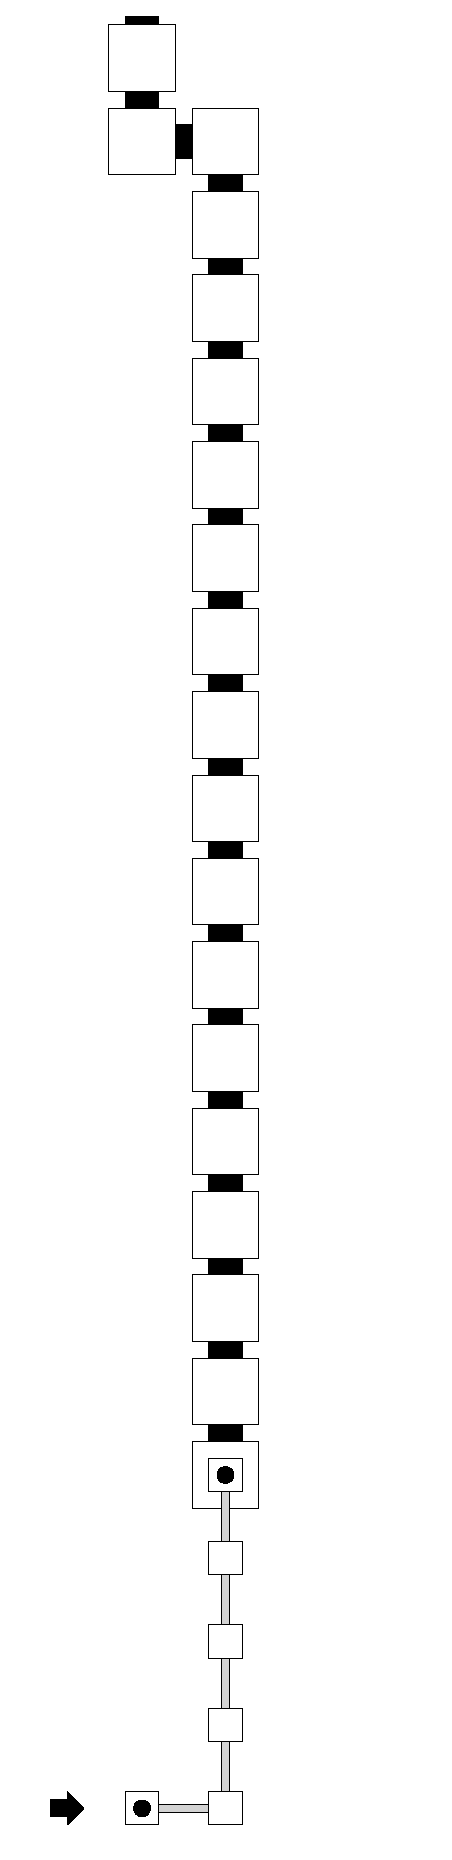
\includegraphics[width=0.45in]{warping_post_warp_case1_digit1_msr}}}%
            ~
            \subcaptionbox{Digit 1 - case 2 overview \label{fig:post_warp_1_op_msr_msd_overview}}
            {\makebox[0.24\textwidth][c]{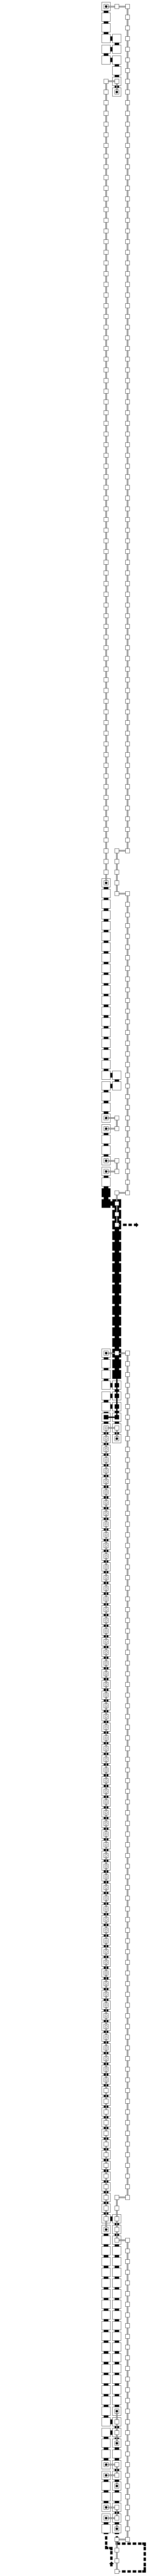
\includegraphics[width=0.45in]{overviews/case1/post_warp_1_op_msr_msd}}}%
            ~
        \end{figure}

        \begin{figure}[H]\ContinuedFloat
            \subcaptionbox{Digit 1 - case 2 \label{fig:post_warp_1_op_msr}}
            {\makebox[0.24\textwidth][c]{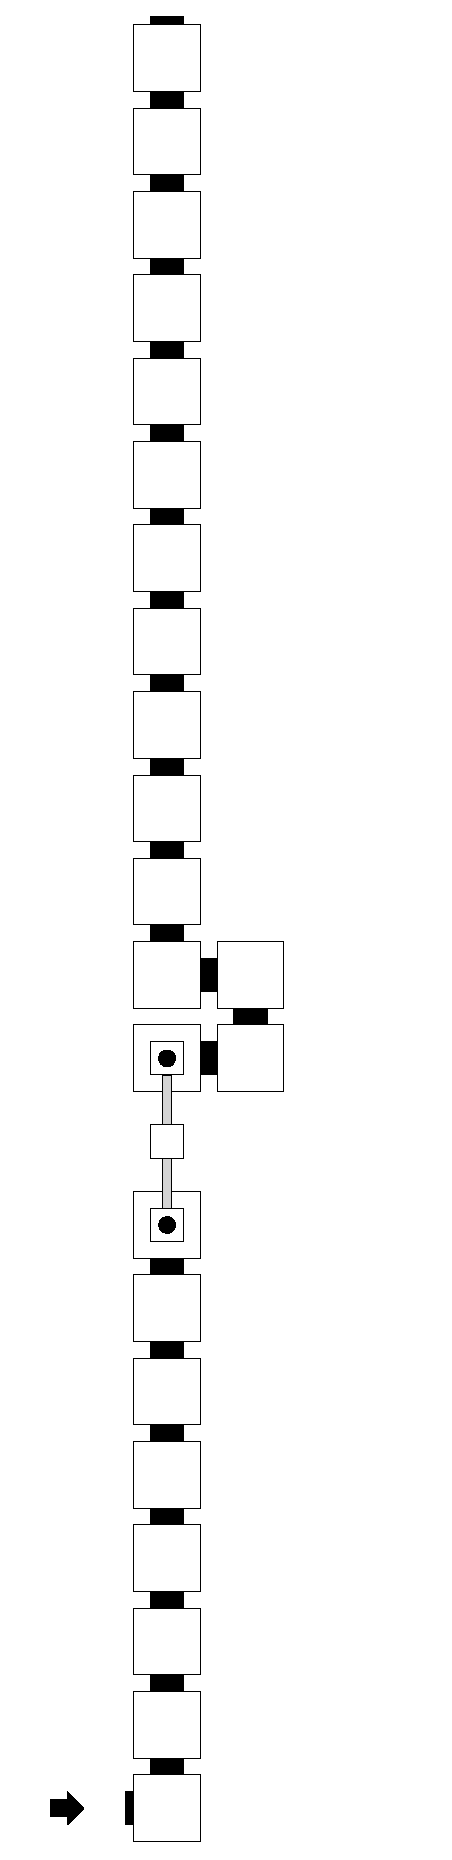
\includegraphics[width=0.45in]{warping_post_warp_case2_digit1_msr}}}%
            ~
            \subcaptionbox{Digit 1 - case 2 overview \label{fig:post_warp_1_op_msr_overview}}
            {\makebox[0.24\textwidth][c]{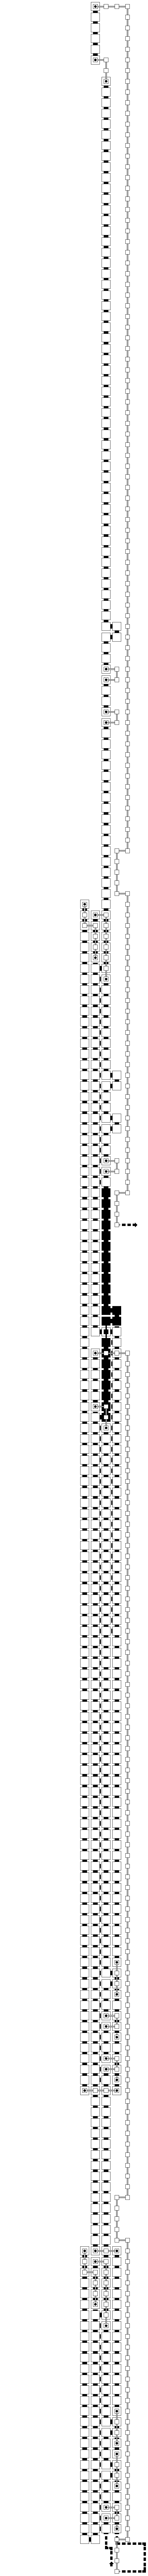
\includegraphics[width=0.45in]{overviews/case2/post_warp_1_op_msr}}}%
            ~
        \end{figure}
        \begin{figure}[H]\ContinuedFloat
            \subcaptionbox{Digit 2 - case 2\label{fig:post_warp_2_op_msr_msd}}
            {\makebox[0.24\textwidth][c]{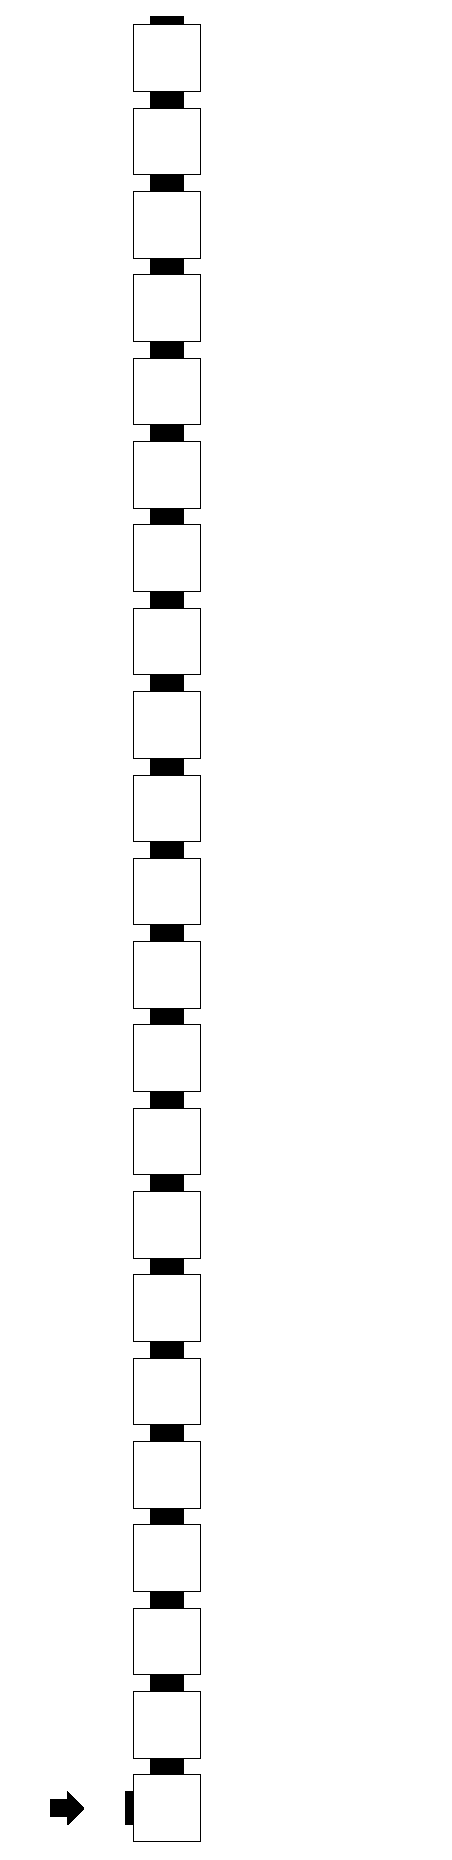
\includegraphics[width=0.45in]{warping_post_warp_case2_digit2_msr}}}%
            ~
            \subcaptionbox{Digit 2 - case 2 overview \label{fig:post_warp_2_op_msr_msd_overview}}
            {\makebox[0.24\textwidth][c]{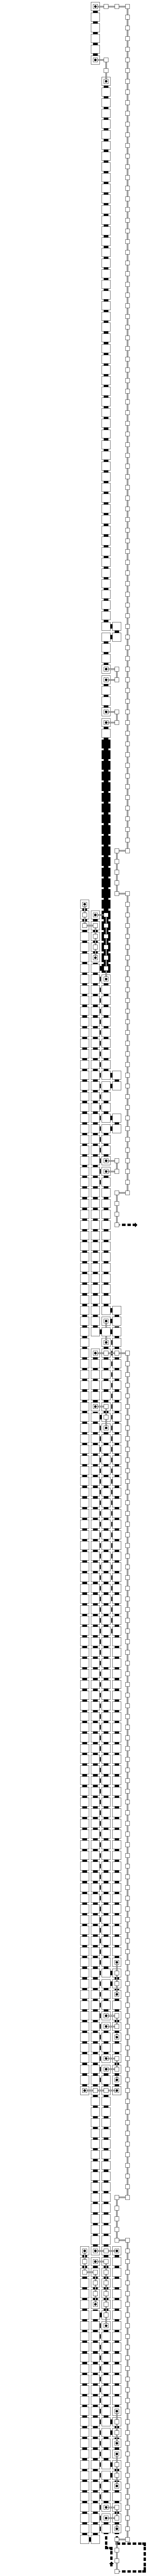
\includegraphics[width=0.45in]{overviews/case2/post_warp_2_op_msr_msd}}}%
            ~
            \subcaptionbox{Digit 2 - case 2 (seed) overview \label{fig:post_warp_2_seed_op_msr_msd_overview}}
            {\makebox[0.24\textwidth][c]{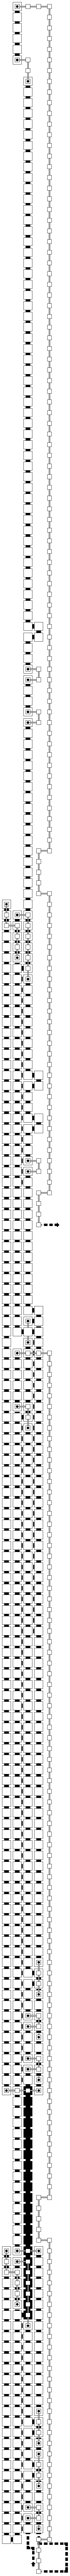
\includegraphics[width=0.45in]{overviews/case2/post_warp_2_seed_op_msr_msd}}}%
            ~
            \caption{\label{fig:post_warp_gadgets} The {\postwarp} gadgets.}
        \end{figure}
    \end{itemize}
